\section{Overview}\label{sec:overview}


Figure~\ref{fig:overview} shows the overview of our algorithm. 
The input 2D layout of a carton consists of a set of cutting edges (solid lines) and folding edges (dashed lines).
%
Given the 2D layout, an undirected graph is built, and a set of polygonal panels are extracted by finding the minimum cycles in the graph, as Figure~\ref{fig:overview}(b) shows. 
Therefore, the 2D layout can be represented by a polymesh $\mathcal{L}=(V,E,P)$, where $V$ is the set of vertexes, $E$ is the set of all edges, and $P$ is the set of panels. 
The edge set $E=E_c\cup E_f$, where $E_c$ is the set of cutting edges, and $E_f$ is the set of folding edges.
%
To build a 3D carton model $\mathcal{M}=(V, E, P)$ from the 2D layout $\mathcal{L}$, which share the same topology, we compute the 3D coordinates of all of the vertexes in $V$. 
%

However, it is not intuitive to analytically define the desired final 3D shape from a 2D layout. 
One possible alternative is to detect all the possible geometric constraints, such as vertex merging, panel parallelism, orthogonality between adjacent panels, and then integrate all these possible constraints together to form a large equation system. 
The challenge is that these local constraints can not adequately describe complicated and creative designs. 
Moreover, there are many ambiguities when detecting these constraints in a 2D layout, such as edges and panels that exist within the same shape. 
%
We propose a two-step algorithm based on the observation that humans usually fold edges at a right angle in order to obtain a rough shape, and then they merge the vertexes or edges to create a stable 3D carton.
% Our algorithm consists of two steps. 
First, an initial 3D model (Figure~\ref{fig:overview}(c)) is constructed based on a specific angle along each folding edge, as described in Sec.~\ref{sec:initialization}.
The user can then manipulate and explore the various 3D shapes of the carton based on a series of suggested operations provided by our system. 
%
The final model is shown in Figure~\ref{fig:overview}(e).
The details of each step are introduced in the following sections. 
 
\begin{figure}
	\centering
	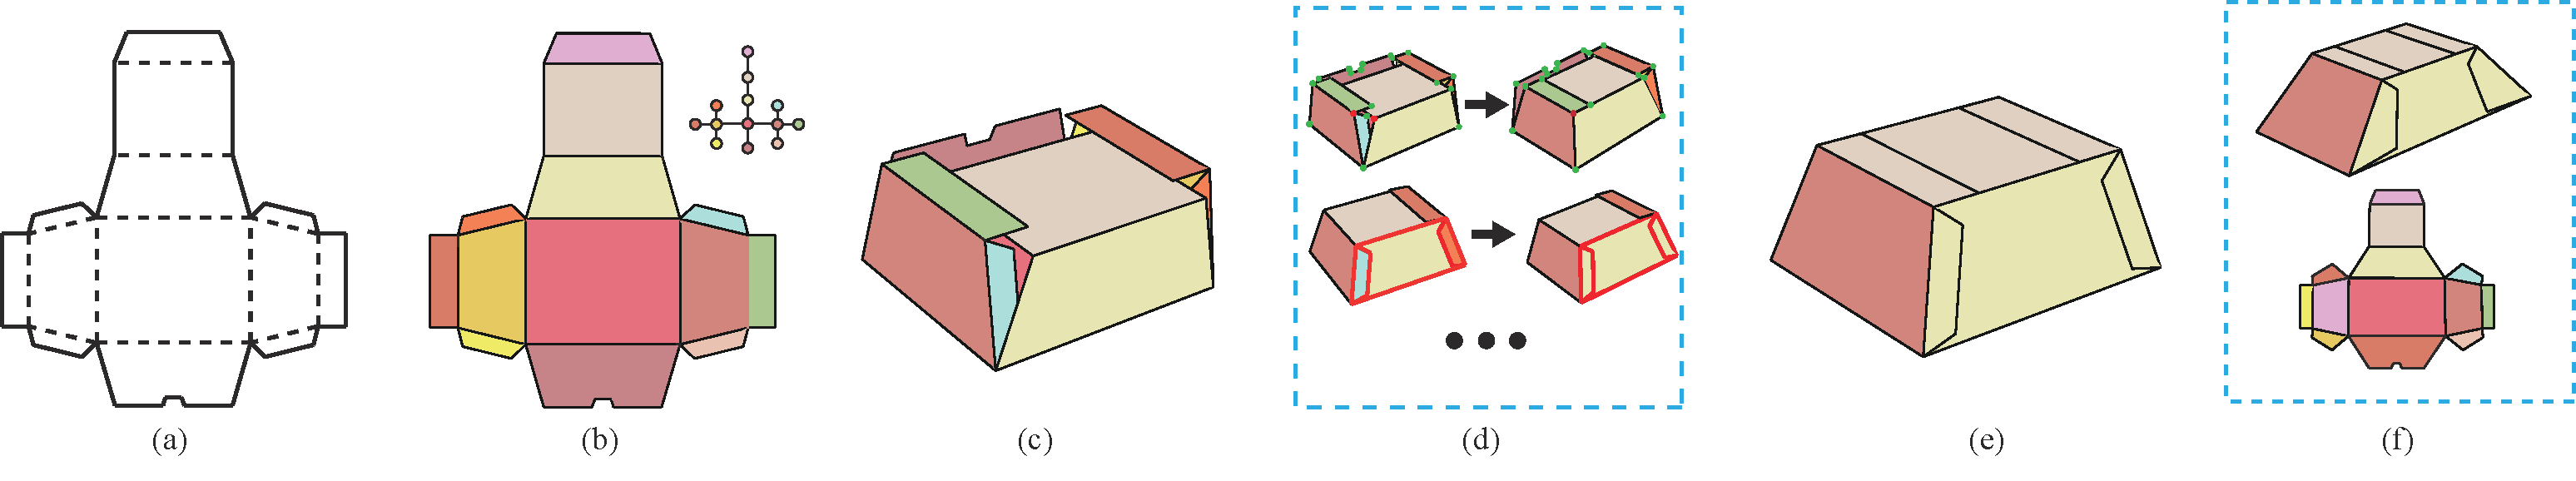
\includegraphics[width=0.9\textwidth]{images/overview}
	\caption{Given a 2D layout (a), we first extract its 2D mesh (b) with different panels in different colors. By providing each folding edge with the same angle, which is $\pi/2$, an initial 3D model can be constructed~(c). The final carton model (e) is built by a shape optimization technique based on a series of suggested geometrical constraints (d).}
	\label{fig:overview}
\end{figure} 
 

